\documentclass[conference]{IEEEtran}
%\usepackage{cite}
\usepackage[pdftex]{graphicx}
%\graphicspath{{images/}}
\DeclareGraphicsExtensions{.pdf}
\usepackage{array}
\usepackage{url}
\usepackage{amsmath}

% correct bad hyphenation here
%\hyphenation{}

\begin{document}
\title{Using Interactive Protocols to Gain Power Savings in Wireless Communication}

\author{\IEEEauthorblockN{Nicholas Farnan and James Larkby-Lahet}
\IEEEauthorblockA{Department of Computer Science, University of Pittsburgh\\ Pittsburgh, PA 15260 -- USA \\ Email: \{nlf4,jamesll\}@cs.pitt.edu}}
\maketitle

\begin{abstract}
As wireless communications allow for devices to be used untethered as long
as their batteries will allow them, saving power in such communications is
becoming increasingly important to their ability to function in their most
independent state. To further the goal of keeping wireless devices in such
a state, we present here an implementation of a protocol proposed by Gagie
to minimize the number of bits transmitted by the sender of some data in a
wireless communication. We provide experimental results to show that our
implementation does, indeed have the potential to save energy under the power
model of real world wireless chipsets.
\end{abstract}

\section{Introduction}

Wireless communication devices are becoming commonplace across many
different application domains.  The characteristics of phone, wifi,
sensor and bluetooth networks and devices are quite diverse, however
several commonalities exist.

Power concerns are common in wireless networks, as we frequently wish
to cut power cords as well as Ethernet cables.  Wireless nodes are
forced to rely on limited battery capacity to provide the maximum
length of availability.  Recharging or replacing batteries ranges from
inconvenient in the case of of personal electronics in the hands of a 
traveler to difficult or impossible in remote sensor network deployments, 
such as jungle and marshland environmental monitoring.

One interesting property of wireless networks that is often exploited
for wireless power management is asymmetry in the power levels of
various network nodes.  At one level, some nodes,
frequently including routers to external networks, are connected to
power mains and do not rely on battery power.  These nodes may be able
to spend more energy in order to reduce energy expenditure in battery
powered nodes, for example by serving as routers for messages between
nodes.

In a potentially cooperative setting, such as sensor networks, the
locked-down networks of cellular carriers or the collaborative WiFi
mesh of the One Laptop Per Child project's XO computer, the global
usefulness of a network can outweigh the individual power hoarding of
nodes.  As cooperative network nodes double as routers for other
nodes' data, it is important to keep as many nodes alive as possible.
In this setting, nodes may develop individual variations in power
level, due to variation in sensing and particularly routing workload.
We may wish to expend more energy on nodes with extra battery life if we
can extend the battery life of more significantly drained nodes.

It is natural that power-aware ad-hoc routing protocols have been
studied to reduce variability in node power levels, thereby extending
the amount of time the network operates at maximum node strength.
This savings may come at the cost of network life during the period of
reduced functionality as node batteries become fully drained, and the
chances of network partition increase dramatically.  These protocols
adjust the optional transmission data.  While messages certainly must
be sent, individual nodes do not necessarily need to participate, and
the choice of participants is the output of the algorithm.

For a given node that is required to transmit data, these algorithms
can reduce the energy cost of transmission, however their sole
mechanism for doing so is the selection of a closer communication
partner for reduced transmission power, and hence energy
consumption.

Given the necessity of a communication in a wireless power-constrained
network, two cases allowing for energy optimization may exist.  We
aimed to address the case where a power-poor node must communicate
with an less energy-constrained receiver.  Specifically, we
investigated the potential for energy savings via interactive
communication, where the receiver may also transmit data to the sender
in an attempt to reduce the number of bits that must be transmitted by
the sender, and hence total energy consumed by the sender.  This is
only possible if the energy required to receive the additional bits is
less than the energy that would have been spent to transmit the
additional bits.  We demonstrate that this is indeed the case for a
variety of real world devices.

In the second case, an energy-rich sender node may attempt to reduce the
energy used by a energy-poor receiver by compressing data or using a
higher transmission rate to reduce the amount of time the receiver
spends receiving data.  There is no incentive to transmit data from
the receiver in this case as it can only increase the amount of energy
consumed; hence we do not address this case with this technique.

The remainder of this paper is structured as follows, Section 2
presents background on the power characteristics of modern wireless
and sensor devices.  Section 3 presents related work.  Section 4
describes our approach.  In Section 5 we present and analyze experimental
results and conclude with Section 6.

\section{Background}

\begin{table*}
\begin{center}
\begin{tabular}{|r|l|l|}
\hline
Chipset & Receive Power (mW) & Transmit Power\\
\hline
\hline
Intel pro2100 & 1386 & 1914\\
\hline
Cisco Aironet & 1000 & 1480\\
\hline
Orinoco & 925 & 1430\\
\hline
Broadcom bcm4326 & 296 & 625\\
\hline
Mica mote & 13.5 & 36 \\
\hline
Motorola Zigbee & 21 & 28\\
\hline
\end{tabular}

\caption{Power consumption of various wireless chips according to the manufacturer}
\label{tab:wireless_power}
\end{center}
\end{table*}

In order to actually achieve power savings by receiving extra data so
that less can be transmitted, a wireless chipset that uses less power to
receive than it does to transmit is required.  Table \ref{tab:wireless_power}
shows the power used in various states of several wireless radio chipsets
\cite{power_management}\cite{intel_g}\cite{broadcom_g}\cite{zigbee}.  The 
Intel, Cisco, and Orinoco chips are all 802.11b/g adapters while the Broadcom
bcm4326 is a system on a chip with 802.11g capability.  The Mica mote and 
Zigbee both use custom radio protocols.

All of these chips, however, use little power to receive data relative to
the amount they require to transmit.  In some cases (such as the Mica mote
and Broadcom chip) this difference is as large as two to one.

We would like to take this opportunity to propose the following general 
power model which we will use in Sections 5 and 6 to evaluate the results 
of our  experiments.  We shall consider any protocol that maintains the 
following inequality to have the potential for saving energy in wireless 
communications:

\begin{equation}
S_o * P_{TX} \geq S_{TX} * P_{TX} + S_{RX} * P_{RX}
\end{equation}

Where $S_o$ is the size of the original file, $S_{TX}$ is the amount of data
transmitted, $S_{RX}$ is the amount of data received, $P_{TX}$ is the power 
used to transmit data, and $P_{RX}$ is the power used to receive data.  Based
off of our observation that the disparity between reception and 
transmission levels can be as large as two to one, we normalize the
previous inequality by dividing by the transmission power.

\begin{equation}
S_o \geq S_{TX} + (\frac{1}{2} * S_{RX})
\end{equation}

\section{Related Work}

In \cite{Adler98}, Adler and Maggs propose that asymmetric
communication channels could be exploited for the purposes of saving
power in wireless transmission.  Their communication model consists of
a client that wishes to send some data drawn from a probability
distribution $D$ to a server, where the server has knowledge of $D$
which the client lacks.  The server uses the asymmetry of
communication channels to send information about D to the client whose
responses can not only effectively communicate the intended data, but
also do so efficiently, minimizing the amount of data actually sent
from the client to the server. They propose protocols that will result
in an expectation of O($n$) bits being sent by the server and
O(H($D$)$ + 1$) bits being sent by the client where $n$ is the number
of bits in the data the client wishes to communicate with the server
and H($D$) being the binary entropy of $D$.  They offer two varieties
of such protocols, one where data is exchanged over some number of
rounds, and another where all communication occur in a single round at
the cost of additional server-side computation.  In both cases, one
round involves a single communication from server to client and
another single response.

This work was followed up by \cite{Watkinson01}, in which Watkinson,
Adler, and Fich provide protocols that result in H($D$)$ + 2$ bits
sent by the client in expectation and $n$(H($D$)$ + 2$)) bits sent by
the server in expectation.  Similar to \cite{Adler98}, the authors
provide both multi-round and single-round variations of their
protocol.  Again, the single-round variant comes at the cost of
additional server-side computation.

All of the above protocols were supplanted by Gagie's work in
\cite{Gagie06} where he showed that any dynamic instantaneous
compression algorithm could be converted to an asymmetric
communication protocol.  The intuition behind this is that Shannon's
theory requires the client to send H(D) bits, which is achieved by the
entropic encoding.  The only relevant information that the server may possess
that the client does not is the distribution observed across many
messages, including those from nodes other than the client.  By
transmitting this distribution, the dynamic instantaneous (one-pass)
encoder starts with a more representative distribution than the
uniform distribution it initially would assume.

Gagie's model of communication also differs from those previously
proposed in that he does not require the server to have pre-existing
knowledge of $D$ and instead accounts for the server acquiring such
knowledge on-line as it receives messages from clients.

The work presented here is an implementation of Gagie's proposed
protocol.  It differs from Gagie's work in \cite{Gagie06} in that we
provide experimental results showing the effectiveness of using
dynamic instantaneous compression algorithms to reduce the amount of
data a client sends in order to communicate a message, as well as the
energy savings that can be gleaned from the use of such a protocol.

\section{Implementation}

In our implemented protocol, the server's representation of $D$ is maintained as
a list of the frequency counts for all symbols in a given alphabet (to encode
a byte at time, the alphabet would consist of [0-255]).  These frequency
are sent to any client who requests to send some data to the server.  Upon 
receiving these frequency counts, the client uses them to perform a range
encoding on the data it wishes to send to the server.  As the client
encodes each symbol in the alphabet, it updates the frequency count for that
symbol accordingly.  Once the client has encoded its message, it sends the
code word for said message to the server, who, whilst decoding the message,
similarly updates its persistent copy of frequency counts as each symbol in
the message is decoded.

We chose range encoding as our entropic compression algorithm, rather
than Huffman Coding as Gagie suggested.  Range encoding produces a
single codeword of output, allowing it to represent symbols using
fractional bits (sharing the remainder with subsequent code words),
and therefore more closely approach H($D$) \cite{range_encoder}.

\section{Results}

\subsection{Experimental Setup}

To perform our experiments, we placed two laptops with Intel Core2Duo
processors and the Intel PRO/Wireless 3945ABG network adapter four feet
apart and connected them via ad-hoc 802.11g.  Both machines were running 
Ubuntu Linux version 8.10.  All measurements of our
experiments were performed on the client.  The client laptop's processor was
running at its full speed of 1.8GHz, though in order to allow for accurate
measure of timing via CPU cycles, we disabled on of it's two cores.  To 
limit the effect of contention for CPU resources during these measurements,
the operating system was booted into single user mode during these experiments
The amount of data transmitted was recorded by statistical instrumentation built
into our test program.  All network traffic was captured through the
tcpdump utility and network latencies were later determined offline from
these dumps.  Latencies are measured as the time from the client sending its
request to transfer a file to sending the last of its data packet.  
Timing measurements in CPU cycles were taken from within our
test program by reading the value of the CPU's RDTSC counter.

We ran our test on the transfer of two ASCII text files, one small (7973 bytes),
and one larger (30173 bytes).  The server description of $D$ was initially
flat, with all symbols given a frequency count of one.  The server maintained
its state across five repeated transfers of the same file, allowing the 
frequency counts to become adjusted to the data being transmitted.  This was 
done to show both the effect of attempting to send data that is not 
particularly well suited to the distribution $D$ (the initial iteration) as 
well as transmitting rather well suited data (later iterations).  All of 
the data presented here has been averaged over 5 repeated trials and is 
shown with 90\% confidence intervals bounding the error of said trials.

\subsection{Experimental Results}

\begin{figure}[!t]
\centering
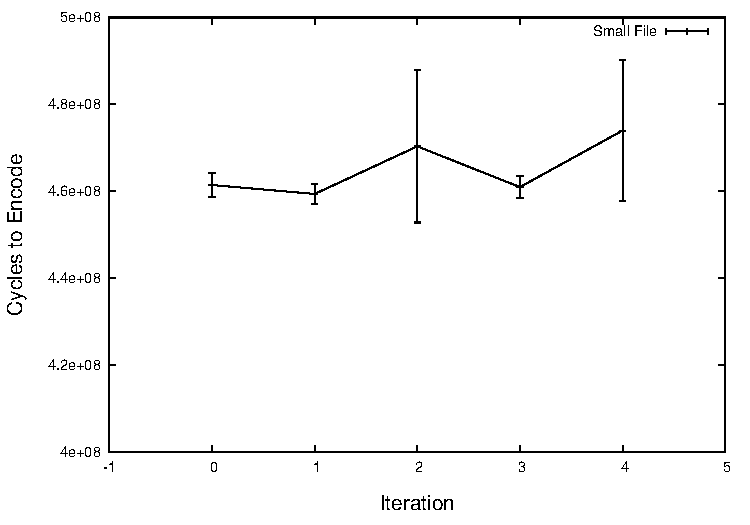
\includegraphics[scale=0.63]{images/sm_cycles.pdf}
\caption{Cycles to Encode the Small File}
\label{fig:sm_cycles}
\end{figure}

\begin{figure}[!t]
\centering
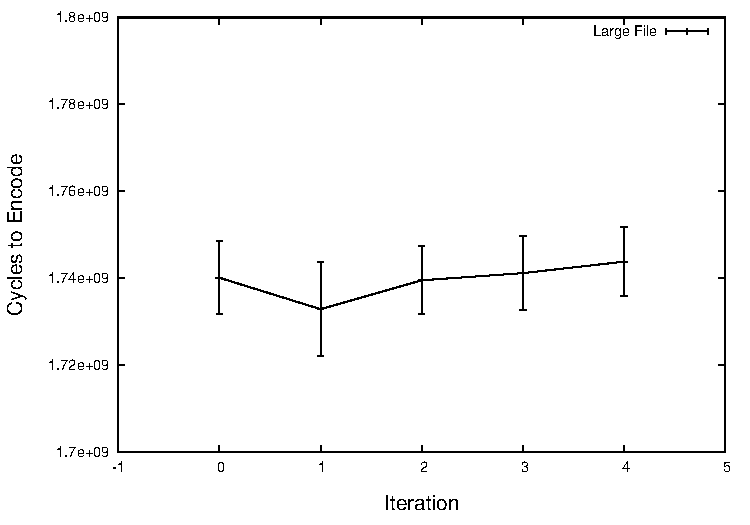
\includegraphics[scale=0.63]{images/lg_cycles.pdf}
\caption{Cycles to Encode the Large File.}
\label{fig:lg_cycles}
\end{figure}

\begin{figure}[!t]
\centering
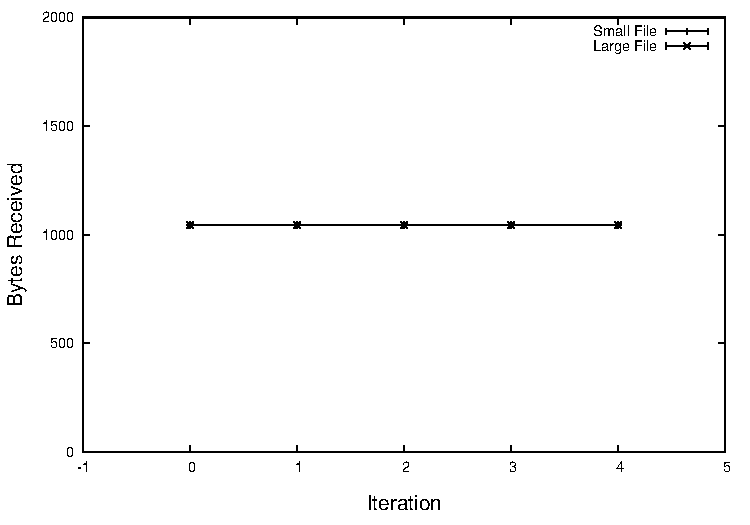
\includegraphics[scale=0.63]{images/rxbytes.pdf}
\caption{Bytes Received}
\label{fig:rxbytes}
\end{figure}

\begin{figure}[!t]
\centering
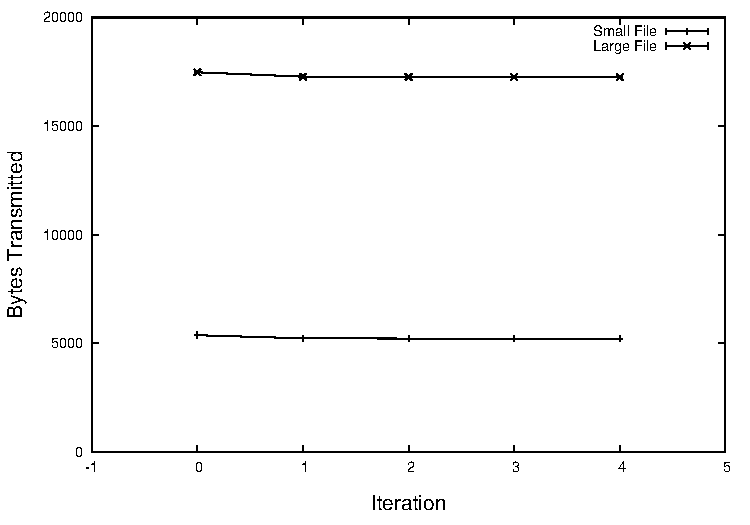
\includegraphics[scale=0.63]{images/txbytes.pdf}
\caption{Bytes Transmitted}
\label{fig:txbytes}
\end{figure}

\begin{figure}[!t]
\centering
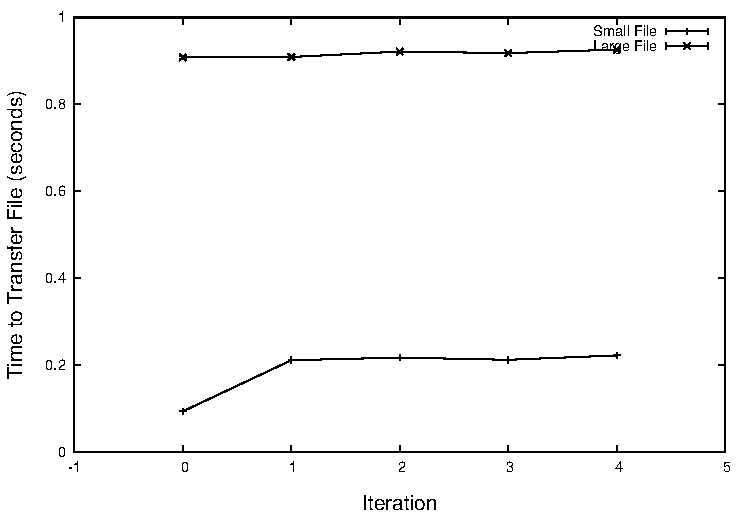
\includegraphics[scale=0.63]{images/latency.pdf}
\caption{Transfer Time (seconds)}
\label{fig:latency}
\end{figure}

Note that our results for the number of bytes received are the same for both 
as no matter the size of the file, we still send an array of 256 unsigned 
integer values that are the frequency counts of symbols seen by the server so
far.  Also of note is the slight drop in bytes transmitted after the first 
iteration of the protocol.  This is due to the dynamic encoder gaining a better
grasp of the distribution $D$ after multiple passes over the same file.  This 
difference is rather muted as since our protocol updates frequency counters
as it encodes the data, the affect of the server sending a poorly-matched 
distribution is mitigated.

Referring back to our previously proposed power model, we find that:

\begin{equation}
7973 \geq 5381 + (\frac{1}{2} * 1044)
\end{equation}

\begin{equation}
7973 \geq 5903
\end{equation}

For the small file and that:

\begin{equation}
30173 \geq 17477 + (\frac{1}{2} * 1044)
\end{equation}

\begin{equation}
30173 \geq 17999
\end{equation}

In the case of the large file.

Our experiments show that our protocol does have the potential to save power
as it maintains our previously defined inequality.

Our cycle counts of time to encode show the amount of work done by the CPU in 
our protocol.  Although file size drastically affects the amount of work done 
to encode, there is no clear trend of an increase or decrease in computational 
complexity for a better or worse matched distribution.

Finally, our latency graphs show the time taken to complete the entire 
communication of a message from client to server.

\section{Conclusion}

We present an approach to conserving power during message
transmission, based on entropic encoding.  Alternative
application-specific approaches such as in network aggregation may be
able to compress more effectively that entropic compression, however
when these approaches cannot be applied or the nature of the
communication is known beforehand our approach is `optimal' in that 
range encoding asymptotically achieves H($D$).

While our approach requires some energy expenditure by the receiver
this cost is constant for a fixed symbol size.  Ultimately the
additional power expended by this reverse transmission will not be the
deciding factor as to whether larger message transceives save power or
not.  Instead the critical comparison appears to be between the
reduction in the number of bits transmitted (and the resulting energy
usage) and the energy consumed by the CPU during compression.  We did
not attempt to optimize our compressor in any way, so the lower bounds
of energy consumption by the compressor remains to be seen.

We have, however, used this protocol to show that potential energy savings 
could be garnished through its use.  We have defined a power model based off
of the power usage of actual wireless radio chipsets, and shown that our 
protocol fits well within the bounds required to save energy in wireless
transmissions.

\bibliographystyle{IEEEtran}
\bibliography{gagie}
\end{document}
